\documentclass[a4paper, british]{article}

\usepackage[utf8]{inputenc}
\usepackage[T1]{fontenc}
\usepackage{babel}
% \usepackage[margin=2.5cm,a4paper]{geometry}
% \usepackage[skip=1em]{parskip}
\usepackage{lmodern} 
\usepackage{microtype}
% \usepackage{xcolor}
\usepackage{graphicx}
\graphicspath{ {./figures/} }
% \usepackage{float}
% \usepackage{enumitem}
\usepackage{adjustbox} % rescale - useful for Dia exported TeX
\usepackage{tikz}
% \usepackage{pgfplots}
\usepackage{booktabs} %tables no vertical lines
% \usepackage{array}
% \usepackage{authblk}
% \usepackage{fancyhdr} %headers and footers
% \usepackage{titlesec}
% \usepackage{tcolorbox} % framed text boxes
% \usepackage{mathtools, amssymb, amsthm}
% \usepackage{gensymb}
\usepackage{chemformula} % chemical formulae
\usepackage{chemfig} % molecular figures
\usepackage{siunitx}
\usepackage{csquotes}
\usepackage[titletoc, title]{appendix}
% \usepackage{lettrine} % initials

\usepackage[
pdfauthor={Adam Menne},
pdftitle={Chemistry 264 - Practical 4},
pdfsubject={},
pdfkeywords={}]{hyperref}

\usepackage[noabbrev]{cleveref}

\usepackage[
backend=biber,
style=numeric,
sorting=none,
doi=true,
isbn=false
]{biblatex}
\addbibresource{citations.bib}

\setlength{\parskip}{1em}
\setlength{\parindent}{0em}
\linespread{1.3}

\title{Chemistry 264\\ Practical 4}
\date{Last editted on \today}
\author{Adam Menne\\ Stellenbosch University}

\begin{document}

\maketitle

\begin{abstract}
\noindent
In this practical a sodium thiosulphate solution was standardised and the percentage hypochlorite of a commercial bleach was determined.
\end{abstract}

\tableofcontents

\newpage

\section{Introduction}

In this practical we carry out a titration in order to standardise a sodium thiosulphate solution using potassium iodate. This solution was then used in a titration to determine the mass percentage hypochlorite in a commercial bleach.

% \begin{figure}[htb]
%     \centering
%     \chemfig{
%         HO% 3
% -[:330,,2]% 1
%            (
%      =[:270]O% 4
%            )
%   -[:30]% 2
%            (
%       =[:90]O% 6
%            )
% -[:330,,,1]OH% 5
% }
% \end{figure}

\section{Results}

\subsection{Part 1}

We find that our titrations for part 1 were relatively consistent, \cref{fig:titration} shows the concentration of \(Na_2S_2O_3\), calculated over seven titrations. These values have a relative standad deviation of 7.951 as can be seen in \cref{table:data}, which also shows the mean and CI values.

\begin{figure}[h]
    \centering
    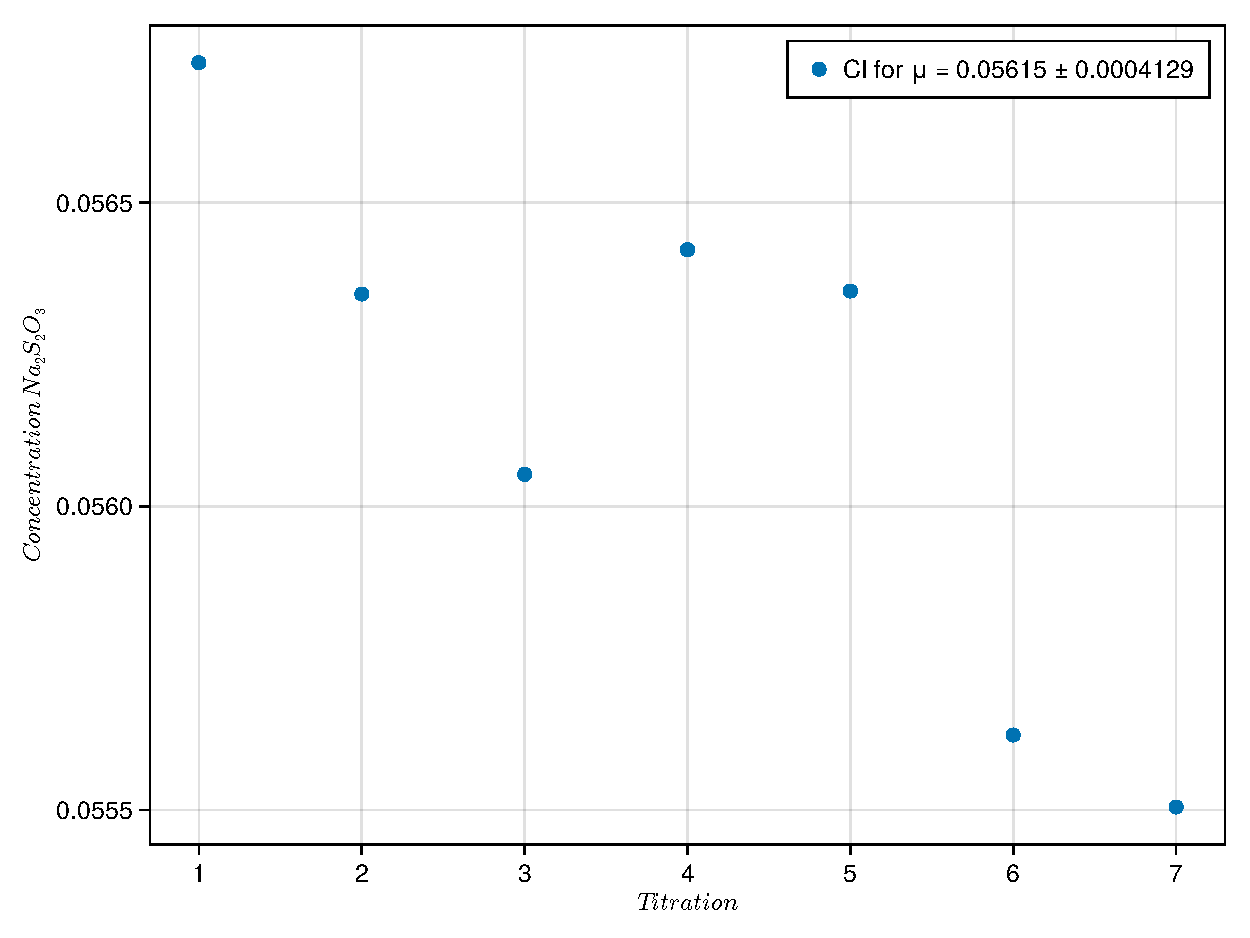
\includegraphics[width=\textwidth]{figures/titration.pdf}
    \caption{Concentration of \(Na_2S_2O_3\)}
    \label{fig:titration}
\end{figure}

\vspace{25mm}

\begin{table}[h]
    \centering
    \caption{Supplementary Data}
    \begin{tabular}{llc}
        \addlinespace
        \toprule
        Mean & RSD & CI\\ 
        \midrule
        0.05615 & 7.951 & 0.05574 - 0.05656\\
        \bottomrule
        \end{tabular}
        \label{table:data}   
\end{table}

\subsection{Part 2}

From the two titrations that were carried out we find that the commercial bleach analysed has a mean percent \(NaOCl\) by mass of 2.948\%

A static export of the notebook containing all analysis and figures is availible at \url{https://adammenne.github.io/chemistry_264/practical_4/notebook.html}. With full source code availble at \url{https://github.com/AdamMenne/chemistry_264/tree/master/practical_4}

\section{Discussion}

From the titrations that were carried out, the metrics of relative standard deviation and confidence intervals for the mean, show that the titrations were consistent and precise for part 1. However in part 2 there is a more substantial deviation between the two titrations carried out 

However improvements are possible by increasing the number of titrations carried out (especially in part two), and utilising a more accurate and precise method of identifying when the equivalence point has been reached.

\newpage

\begin{appendices}

\section{Flow diagram}

\subsection*{Part 1}

\begin{enumerate}
    \item Weigh out \(\sim\) 0.355\(g\) \(KIO_3\), prepare 200 \(cm^3\) solution.
    \item Add 5\(cm^3\) of 5\% \(KI\) solution and 10\(cm^3\) 0.5\(M\ H_2SO_4\) to a Erlenmeyer flask.
    \item Fill a burette with the \(KIO_3\) solution, and another with thiosulphate solution
    \item Tap \(\sim\) 5 \(cm^3\) \(KIO_3\) into flask, the solution will turn yellow-brown. Tap thiosulphate until the solution is close to colourless. Repeat until 25-30\(cm^3\) of each solution has been used.
    \item Add 2 \(cm^3\) of starch indicator
    \item Titrate until the solution has become colourless
    \item Titrate using double-burette technique, tabulating data.
\end{enumerate}

\subsection*{Part 2}

\begin{enumerate}
    \item Tap 5 \(cm^3\) bleach solution into an Erlenmeyer flask
    \item Add 50 \(cm^3\) distilled water
    \item Add 10 \(cm^3\) 6\(M\) acetic acid
    \item Stir well, and add 10 \(cm^3\) 2\(M\) potassium iodide
    \item Fill a burette with the thiosulphate solution, and Titrate
    \item Repeat procedure once more
\end{enumerate}

\newpage

\section{MSDS}

\subsubsection*{Potassium iodate}

\begin{itemize}
    \item Oxidising, corrosive, harmful
    \item[-] avoid contact with eyes
    \item[-] may intensify fires
    \item[-] do not ingest 
    \item[-] if in eyes, wash continuously for several minutes
\end{itemize}

\subsubsection*{Potassium iodide}

\begin{itemize}
    \item Irritant, health hazard, environmental hazard
    \item[-] avoid contact with skin and eyes, do not inhale or ingest
    \item[-] wash immediately if contact occurs
\end{itemize}

\subsubsection*{Hydrochloric acid}

\begin{itemize}
    \item Corrosive, harmful
    \item[-] may cause skin burns, eye damage and respiratory irritation, do not inhale
    \item[-] if in contact with skin or eyes wash for several minutes
\end{itemize}

\subsubsection*{Sodium thiosulphate}

\begin{itemize}
    \item Harmful
    \item[-] causes skin, eye, and respiratory irritation
    \item[-] if in contact with skin or eyes wash for several minutes
\end{itemize}

\subsubsection*{Sodium hypochlorite}

\begin{itemize}
    \item Corrosive, environmental hazard
    \item[-] may cause skin burns, and eye damage, do not ingest or inhale
    \item[-] if in contact with skin or eyes wash for several minutes
\end{itemize}

\subsubsection*{Acetic acid}

\begin{itemize}
    \item Flammable, corrosive
    \item[-] may cause skin burns, and eye damage, do not ingest 
\end{itemize}
    
\end{appendices}

\end{document}